%!TEX root = Slic3r-Manual.tex

\paragraph{Netfabb Studio} % (fold)
\label{par:netfabb_studio}
Netfabb produit une gamme d'applications de mod\'elisation 3D, y compris une version de base gratuite\footnote{http://www.netfabb.com/basic.php}.  Cette version comprend un module de r\'eparation de maillage qui peut aider \`a \'eliminer les diff\'erents probl\`emes rencontr\'es. Les instructions mise \`a jour peuvent \^etre trouv\'es sur le wiki Netfabb\footnote{http://wiki.netfabb.com/Part\_Repair}, ce qui suit est un bref aperçu des \'etapes \`a suivre.

\begin{figure}[H]
\centering
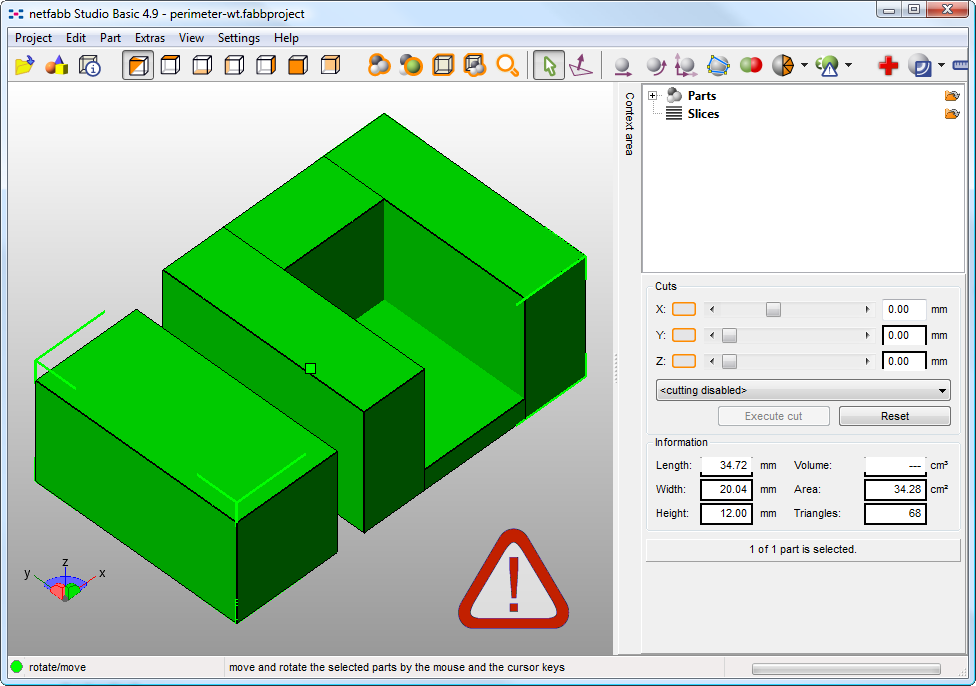
\includegraphics[keepaspectratio=true,width=0.75\textwidth]{working_with_models/netfabb_studio_part_repair.png}
\caption{Netfabb Studio: R\'eparation de mod\`ele.}
\label{fig:netfabb_studio_part_repair}
\end{figure}

\begin{itemize}
	\item Lancer Netfabb studio, et charger le fichier STL qui a un probl\`eme, que ce soit par l'interm\'ediaire du menu \texttt{File} ou par glisser-d\'eposer sur l'espace de travail. Si Netfabb d\'etecte un probl\`eme, il affiche un signe d'alerte rouge dans le coin en bas \`a droite.
	\item Pour ex\'ecuter les scripts de r\'eparation, s\'electionnez la partie et puis cliquez sur la premi\`ere ic\^one d'aide dans la barre d'outils (la croix rouge), ou s\'electionnez dans le menu contextuel \texttt{Extras->Repair Part}.  Cela va ouvrir l'onglet r\'eparation de mod\`ele et de montrer l'\'etat du mod\`ele.
	\item Les onglets \texttt{Actions} et \texttt{Repair scripts} offrent plusieurs scripts de r\'eparation qui peuvent \^etre appliqu\'ees manuellement, mais dans le but de cet aperçu s\'electionez le script \texttt{Automatic repair} corrigera la plupart des probl\`emes.
	\item Le bouton de r\'eparation automatique pr\'esente deux options: par d\'efaut et simples. Choisir par d\'efaut couvrira la plupart des cas. Selectionnez \texttt{execute} pour lancer le script.
	\item Une fois la pi\`ece r\'epar\'ee les r\'eparations doivent \^etre appliqu\'ees en s\'electionnant \texttt{Apply repair}, choisissant s'il faut passer outre la partie existante ou non.
	\item La pi\`ece peut ensuite \^etre export\'e en s\'electionnant \texttt{Export part->As STL} \`a partir du menu contextuel.
	\item Si Netfabb d\'etecte encore que la partie export\'ee contient des erreurs, alors il offrira la possibilit\'e d'appliquer d'autres r\'eparations avant de l'exporter.
	\begin{figure}[H]
	\centering
	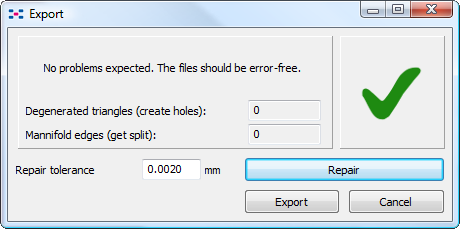
\includegraphics[keepaspectratio=true,width=0.75\textwidth]{working_with_models/netfabb_studio_export_part.png}
	\caption{Netfabb Studio: Export de pi\`ece.}
	\label{fig:netfabb_studio_export_part}
	\end{figure}
\end{itemize}
% paragraph netfabb_studio (end)

\paragraph{Netfabb Cloud Service} % (fold)
\label{par:netfabb_cloud_service}
Netfabb accueille \'egalement un service web o\`u un fichier STL peut \^etre t\'el\'echarg\'e pour \^etre v\'erifi\'e et r\'epar\'e\footnote{http://cloud.netfabb.com/}.  

\begin{figure}[H]
\centering
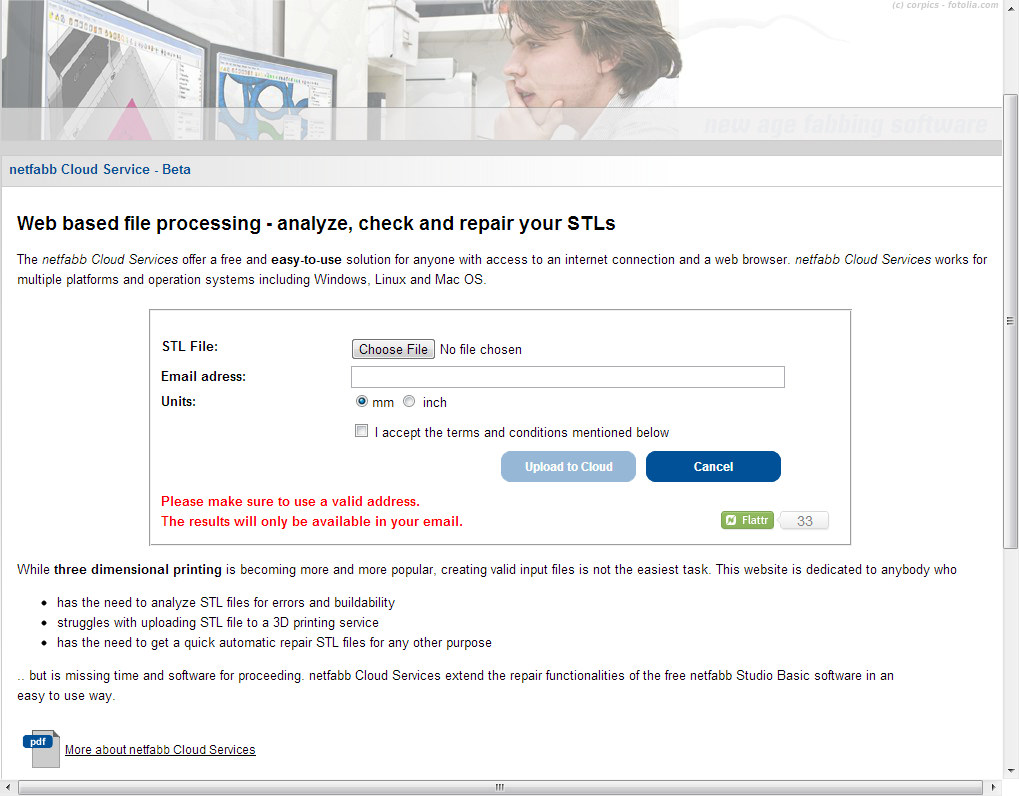
\includegraphics[keepaspectratio=true,width=0.75\textwidth]{working_with_models/netfabb_cloud_services.png}
\caption{Netfabb Cloud Services.}
\label{fig:netfabb_cloud_services}
\end{figure}

\begin{itemize}
	\item Acc\'edez \`a http://cloud.netfabb.com
	\item Choisissez le fichier STL \`a t\'el\'echarger en utilisant le bouton pr\'evu.
	\item Une adresse e-mail doit \^etre donn\'ee pour vous informer quand la prestation est termin\'e.
	\item Choisissez entre les mesures m\'etriques ou imp\'eriales qui doivent \^etre utilis\'es.
	\item Lisez et acceptez les conditions de service, puis cliquez sur \texttt{Upload to Cloud}.
	\item Une fois que le service a analys\'e et r\'epar\'e le fichier, un email est envoy\'e, fournissant le lien de t\'el\'echargement du fichier r\'epar\'e.
\end{itemize}
